\documentclass[11pt]{article}

\usepackage{latexsym}
\usepackage{graphicx}
\usepackage{amssymb}
\usepackage{amsthm}
\usepackage{enumerate}
\usepackage{amsmath}
\usepackage{cancel}
\numberwithin{equation}{section}
\numberwithin{figure}{section}
\numberwithin{table}{section}

\setlength{\evensidemargin}{.25in}
\setlength{\oddsidemargin}{-.25in}
\setlength{\topmargin}{-.75in}
\setlength{\textwidth}{6.5in}
\setlength{\textheight}{9.5in}
\newcommand{\due}{March 18th, 2010}
\newcommand{\HWnum}{7}
\newcommand{\grad}{\bold\nabla}
\newcommand{\vecE}{\vec{E}}
\newcommand{\scrptR}{\vec{\mathfrak{R}}}
\newcommand{\kapa}{\frac{1}{4\pi\epsilon_0}}
\newcommand{\unit}[1]{\ensuremath{\, \mathrm{#1}}}

\begin{document}
\begin{titlepage}
\setlength{\topmargin}{1.5in}
\begin{center}
\Huge{Physics 3320} \\
\LARGE{Principles of Electricity and Magnetism II} \\
\Large{Professor Ana Maria Rey} \\[1cm]

\huge{Homework \#\HWnum}\\[0.5cm]

\large{Joe Becker} \\
\large{SID: 810-07-1484} \\
\large{\due} 

\end{center}

\end{titlepage}



\section{Introduction}
A junction gate field-effect transistor, JFET, uses a bias voltage to control current flow through the transistor. This effect has many applications, but for this Lab we will use the JFET to amplify a signal.

\section{JFET Output Characteristics}
\subsection{Theory}
For a JFET the voltage difference between the gate and the source $V_{GS}$ controls the current flow from the drain to the source, $I_D$. As the drain-source voltage increases the drain current reaches a saturation point called the saturated drain source current. This is where the curve levels out as seen in figure \ref{JFEToutput}.
\begin{figure}[h]
\centering
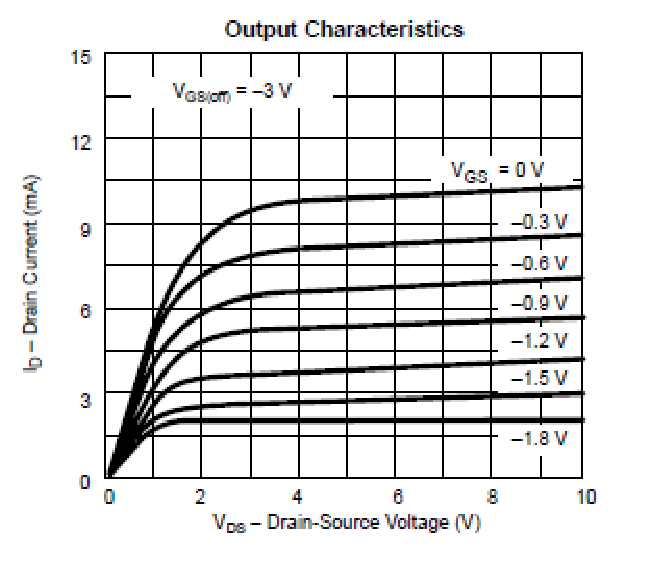
\includegraphics[scale=0.60]{JFEToutput.eps}
\caption{\textit{The output characteristics for the 2N4416a JFET}}
\label{JFEToutput}
\end{figure} 
Note that figure \ref{JFEToutput} has a $V_{GSoff}$ point of $-3\unit{V}$. Where $V_{GSoff}$ is the value for the voltage $V_{GS}$ when the drain current is zero.

Now we can define a value called \emph{transconductance} with a variable $g_{fs}$. The transconductance relates the cahnge in the drain current when the gate voltage is varied slightly, mathematically we say
\begin{equation}
g_{fs}\equiv\frac{\delta I_D}{\delta V_{GS}}
\label{TransCon}
\end{equation}
Usually we find $\delta I_D$ and $\delta V_{GS}$ from plots like the plot in figure \ref{JFEToutput}. Note that $g_{fs}$ is in units of Siemens which is denoted as $\unit{S} = \unit{\Omega^{-1}}$. 

\subsection{Experiment}
To begin the experiment we built the circuit show in figure \ref{Part1JfetSchem} where the resistor labeled ``$k\unit{k\Omega}$''
\begin{figure}[h]
\centering
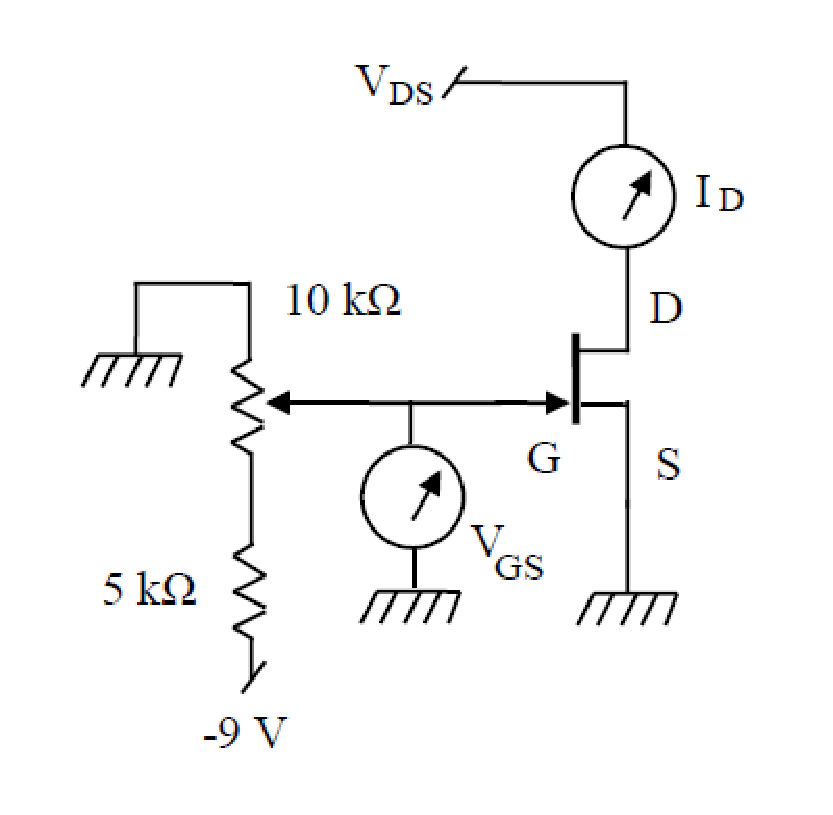
\includegraphics[scale=0.50]{Part1JfetSchem.eps}
\caption{\textit{The schematic for the circuit built to test the JFET output characteristics}}
\label{Part1JfetSchem}
\end{figure} 
 was 2 resistors in series with a total resistance of $4.88\unit{k\Omega}$ and the $-9\unit{V}$ voltage source was supplied by a 9-volt battery with a emf of $-9.45\unit{V}$. For $V_{DS}$ we connected the DC power supply to the circuit with an amp-meter reading the current flow from the DC power supply. This was how we measured $I_D$. To measure $V_{GS}$ we connected the voltage difference to the oscilloscope. Now we can find the relation between $V_{DS}$ and $I_D$. To do this we adjusted the potentiometer until we saw that $V_{GS}=0.0\unit{V}$ on the oscilloscope. Then we adjusted the DC power supply to output different voltages between $0\unit{V}$ and $15\unit{V}$ we recored the resulting values of the drain current. We repeated this for $V_{GS}=-0.1\unit{V}$ and $V_{GS}=-0.2\unit{V}$, the resultant data is in table \ref{OutputData}.
\begin{table}[h]
\centering
\begin{tabular}{c|ccc}
&\multicolumn{3}{c}{Drain Current ($I_D$)}\\
 $V_{DS}$	&$V_{GS} = 0.0\unit{V}$	&$V_{GS} = -0.1\unit{V}$	&$V_{GS} = -0.2\unit{V}$\\
\hline
$0.0\unit{V}$	&$-0.03\unit{mA}$	&$-0.06\unit{mA}$	&$-0.06\unit{mA}$\\
$1.5\unit{V}$	&$5.67\unit{mA}$	&$5.56\unit{mA}$	&$5.07\unit{mA}$\\
$3.0\unit{V}$	&$6.87\unit{mA}$	&$6.40\unit{mA}$	&$5.96\unit{mA}$\\
$6.0\unit{V}$	&$7.12\unit{mA}$	&$6.65\unit{mA}$	&$6.18\unit{mA}$\\
$9.0\unit{V}$	&$6.96\unit{mA}$	&$6.64\unit{mA}$	&$6.19\unit{mA}$\\
$12.0\unit{V}$	&$6.89\unit{mA}$	&$6.56\unit{mA}$	&$6.15\unit{mA}$\\
$15.0\unit{V}$	&$6.77\unit{mA}$	&$6.47\unit{mA}$	&$6.07\unit{mA}$\\
\end{tabular}
\caption{\textit{Drain currents, $I_D$, for different drain voltages, $V_{DS}$. We found this relation for $V_{GS}=0.0,-0.1,-0.2\unit{V}$.}}
\label{OutputData}
\end{table}
We then plotted this data so that we could get the output characteristics of this JFET in figure \ref{PlotJfetOutput}.
\begin{figure}[h]
\centering
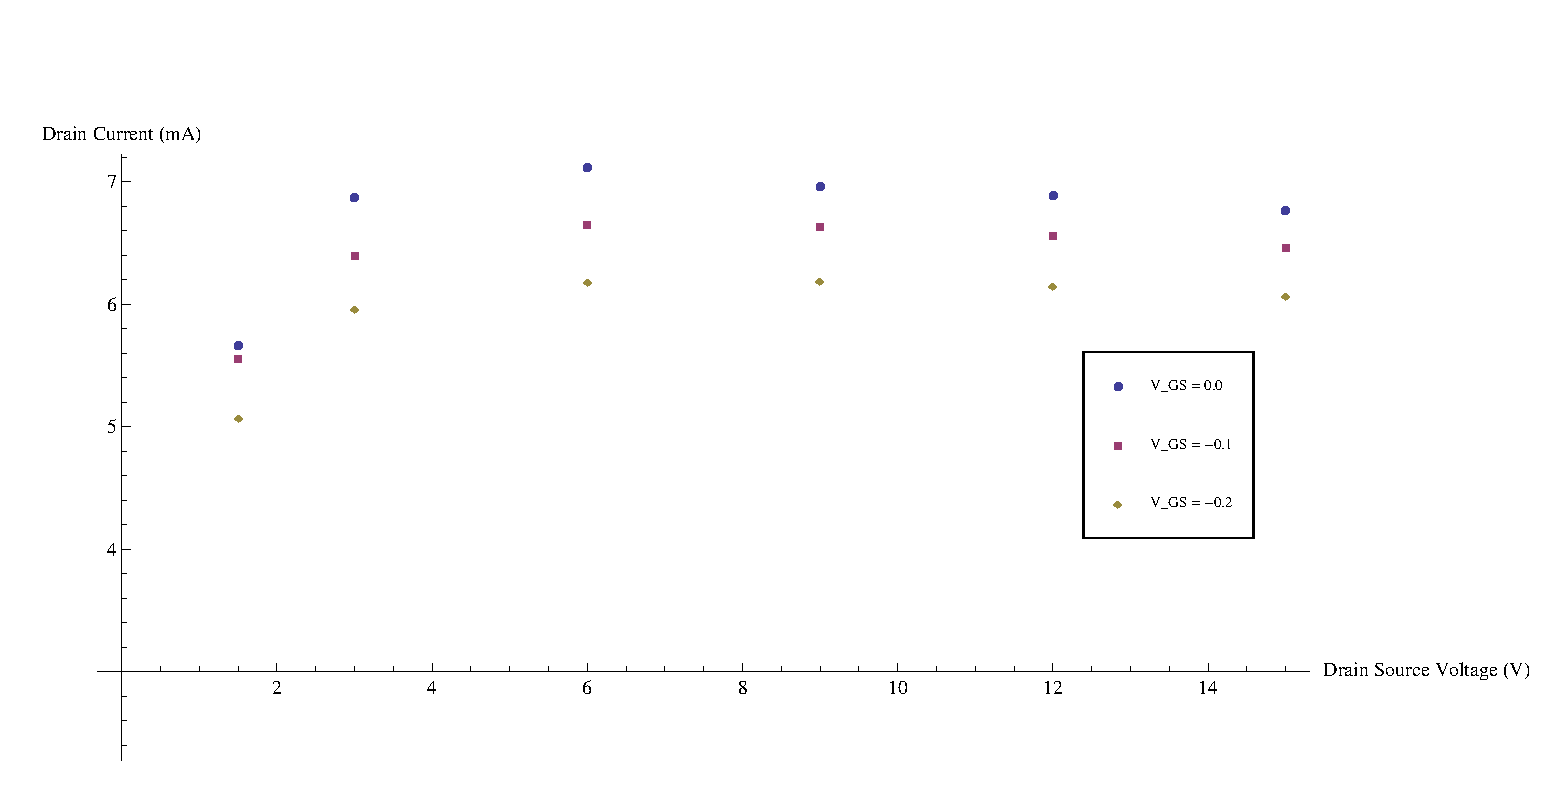
\includegraphics[scale=0.70]{PlotJfetOutput.eps}
\caption{\textit{Plot of the data in table \ref{OutputData}.}}
\label{PlotJfetOutput}
\end{figure} 
Next we measured $V_{GSoff}$. To do this we put set the drain voltage to $10\unit{V}$. We picked a $V_D$ high enough so we had a saturated drain source current. Then we adjusted the potentiometer until we found that $I_D=0$ at this point we read that $V_{GSoff} = -2.2\unit{V}$ from the oscilloscope. Next to find the value of $I_{DSS}$ we adjusted the potentiometer until $V_{GS}=0\unit{V}$ and then we set $V_D=15\unit{V}$ on the DC power supply. The amp-meter read $I_{DSS}=7.08\unit{mA}$.

Now we use the plot in figure \ref{PlotJfetOutput} to find $g_{fs}$ by saying that $\delta I_D=-0.91\unit{mA}$ and $\delta V_{GS} = -0.2\unit{V}$ at $V_{DS}=+3\unit{V}$ and $\delta I_D=-0.70\unit{mA}$ and $\delta V_{GS} = -0.2\unit{V}$ at $V_{DS}=+15\unit{V}$. So equation \ref{TransCon} yeilds $g_{fs} = 4.6\unit{mS}$ for $V_{DS}=+3\unit{V}$ $g_{fs} = 3.5\unit{mS}$ for $V_{DS} = +15\unit{V}$. From the data sheet for the 2N4416a JFET we expect that $g_{fs} = 5.3\unit{mS}$, but this was for $V_{GSoff}=-3\unit{V}$. So we see that our measured result is reasonably close to the expected value.

\section{Common-Source Amplifier}
\subsection{Theory}
The Common-Source Amplifier is shown in figure \ref{CSAmpSchem}. 
\begin{figure}[h]
\centering
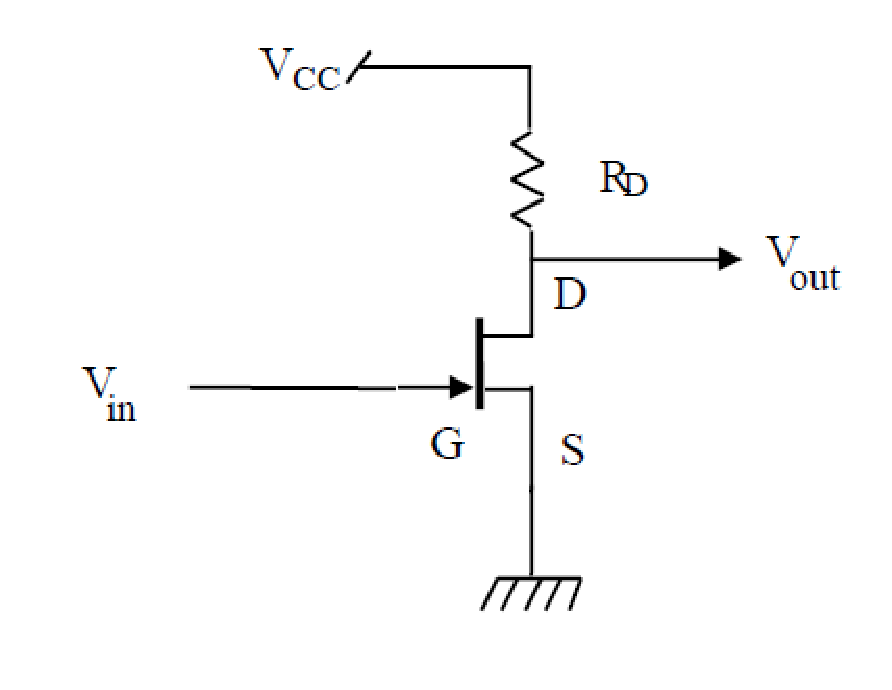
\includegraphics[scale=0.50]{CSAmpSchem.eps}
\caption{\textit{The schematic for the Common-Source Amplifier}}
\label{CSAmpSchem}
\end{figure} 
We see from the schematic that the gain of this amplifier is given by
\begin{equation} 
G = -g_{fs}R_D
\label{Gain} 
\end{equation} 
where $g_{fs}$ is defined by equation \ref{TransCon}.

\subsection{Experiment}
For this part we constructed the circuit in figure \ref{CSAmpSchem} where $V_{CC}$ was two 9-volt batteries with a voltage of $18.9\unit{V}$. Where we picked $R_D$ so that $V_{DS}=+3\unit{V}$ at $V_{GS}=0\unit{V}$. To do this we used figure \ref{PlotJfetOutput} to find that $I_D = 6.95\unit{mA}$ at $V_{DS}=+3\unit{V}$ and $V_{GS}=0\unit{V}$. Then we calculated the voltage drop across $R_D$ as $15.9\unit{V}$. With this and $I_D=6.95\unit{mA}$ and ohm's law we calculated $R_D=2.3\unit{k\Omega}$. In actuality we used $R_D=2.09\unit{k\Omega}$ as that was the value of the resistor that was closest to the value we wanted. 

Next we sent a $1\unit{kHz}$ sine wave into the circuit. We measured the output and input voltage amplitudes using the oscilloscope and found $V_{in} = 0.304\unit{V}$ and $V_{out}=2.42\unit{V}$. So the gain we measured is $G=-7.96$ note that the gain is negative because the signal is inverted. Using $g_{fs}=3.5\unit{mS}$ and $R_D=2.09\unit{k\Omega}$ and equation \ref{Gain} we see that we expect $G=-7.32$ so our measured value is close to the expected value. 

\section{Thermal Noise of a Resistor}
\subsection{Theory}
Inside of resistors there is random motion of the atoms. This causes thermal noise, this is an extra voltage that is created in the resistor. This value is generally very small and is given by
$$V_{rms} = \sqrt{4kTR\Delta f}$$
where $T$ is the temperature in kelvin and $k$ is Boltzmann Constant. We see that the voltage is dependent on the frequency of so if we divide out by that we get
\begin{equation}
v_{th} = \sqrt{4kTR}
\label{Noise}
\end{equation}
note that the units of $v_{th}$ are in $\unit{V}/\unit{\sqrt{Hz}}$. It is also important to note that the noise of two resistors is their individual $v_{th}$ added in quadrature so
$$v_3 = \sqrt{(v_1)^2+(v_2)^2}$$


\subsection{Experiment}
To begin we sent a $1\unit{kHz}$ sine wave into the lock-in amplifier. Then we shorted the clips we had running out of the lock-in A input. We did this to find the internal noise of the lock-in. We found that the noise was $24\unit{nV}$ but we had a $10\unit{kHz}$ bandwidth so $v_{th} = 7.6\unit{nV/\sqrt{Hz}}$


The noise in a resistor is very small. To correct this we will amplify the signal using the common-source amplifier. So we need to find the thermal noise of just the common-source amplifier so we removed the ground from the source input of the JFET and attached the positive input of the clip to the gate of the JFET and the negative lead to ground. Note that this is the only ground in the circuit. Next we shorted the drain and the source and found the noise of the input of the JFET is $158.8\unit{nV}$ note we found this value by taking 10 readings at an even interval and found the average value. So if we divide by the bandwidth we measured $v_{th} = 50.2\unit{nV/\sqrt{Hz}}$. 
But we need to account for the gain to find the actual thermal noise. We measured $G=7.96$ so if we divide by $G$ we will find that $v_{th} = 6.3\unit{nV/\sqrt{Hz}}$. Now if we take this value and the thermal noise of the lock-in and add them in quadrature we see that the total background noise for this circuit is $v_{back} = 9.9\unit{nV/\sqrt{Hz}}$

Now we remove the short between the source and drain. Then we placed a resistor that shorted the source and the where $R=5.00\unit{k\Omega}$. We measured the output noise at lock-in as $471\unit{nV}$ again we divide by the bandwidth and to get $v_{th} = 149\unit{nV/\sqrt{Hz}}$. Now if we take into account the gain of $7.96$ the actual noise is $v_{th} = 18.7\unit{nV/\sqrt{Hz}}$. But this also includes the noise from the JFET and the lock-in amplifier so we need to subtract $v_{back}=9.9\unit{nV/\sqrt{Hz}}$ off in quadrature. So the thermal noise of the $5\unit{k\Omega}$ resistor is $v_{th}=15.9\unit{nV/\sqrt{Hz}}$. If we assume that we are at $300\unit{K}$ with $R=5.00\unit{k\Omega}$ we see that equation \ref{Noise} gives us an expected value of $v_{th} = 9.1\unit{nV/\sqrt{Hz}}$. This value is significantly off of the value we measured, this is due in part to the assumption that the temperature was $300\unit{K}$, but the large part of the discrepancy is due inconsistencies in the lock-in amplifier.

\section{Conclusion}
We see that with the JFET we can amplify a signal. In this case we amplified the thermal noise of a resistor. While the JFET cannot have as large of a gain as an op-amp the gain is still useful and does not require any feedback loops to keep the signal stable. These are advantages when large gains are not your aim.
\end{document}

